\begin{tiny}(Ccu01)\end{tiny} Comme il s'agit de discuter sur le paramètre $m$, le résultat doit être de la forme suivante
\begin{itemize}
 \item Si $m$ ceci alors l'ensemble des solutions est ...
 \item Si $m$ cela alors l'ensemble des solutions est ...
\end{itemize}
\emph{Il ne doit JAMAIS apparaitre quelque chose du genre \og Si $x$ ceci alors ...\fg}\newline
On doit transformer l'équation ou l'inéquaion proposée en une autre équivalente et d'une forme plus commode pour la résolution.

\begin{center}
\'Etude de l'équation $(1)$.  
\end{center}
On peut discuter et répondre directement
\begin{itemize}
 \item Si $m = -1$ l'ensemble des solutions est vide
 \item Si $m \neq 1$  alors l'ensemble des solutions est
\begin{displaymath}
 \left\lbrace \frac{m-2}{m+1}\right\rbrace 
\end{displaymath}
\end{itemize}

\begin{center}
  \'Etude de l'inéquation $(2)$.
\end{center} 
On transforme l'inéquation 
\begin{multline*}
 (2)\Leftrightarrow
\frac{m}{x-1}-\frac{1}{x+2}\leq 0\Leftrightarrow
\frac{m(x+2)-(x-1)}{(x-1)(x+2)}\leq 0 \\
\Leftrightarrow
\frac{(m-1)x+2m+1}{(x-1)(x+2)}\leq 0
\end{multline*}
Lorsque $m-1\neq 0$, on peut factoriser encore et tout revient à placer 
\begin{displaymath}
 h(m) = \frac{1+2m}{1-m}
\end{displaymath}
par rapport à $-2$ et $1$. On étudie la fonction $h$ ainsi définie. Il s'agit d'une fonction \emph{homographique} dont les propriétés suivantes doivent être connues.\newline
On peut la décomposer
\begin{displaymath}
 h(m) = \frac{1+2(m-1)+2}{1-m}
= -2 + \frac{3}{1-3}
\end{displaymath}
\begin{figure}[h!]
 \centering
 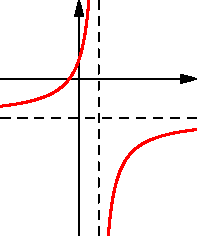
\includegraphics{./Ccu01_1.pdf}
 % Ccu1_1.pdf: 0x0 pixel, -2147483648dpi, 0.00x0.00 cm, bb=
 \caption{Exercice \ref{Ecu1}: graphe de $h$}
 \label{fig:Ccu1_1}
\end{figure}
Son graphe (figure \ref{fig:Ccu1_1}) est une hyperbole et elle est strictement croissante dans chaque intervalle de définition. De plus $h(m)=0$ est impossible et $h(m)=1\Leftrightarrow m=0$.
Tout revient à étudier le signe de
\begin{displaymath}
 (m-1)\frac{x-h(m)}{(x-1)(x+2)}
\end{displaymath}
\begin{itemize}
 \item Si $m\leq 0$: $(m-1)<0$, $-2<h(m)\leq 1$. L'ensemble des solutions est
\begin{displaymath}
 \left] -2,h(m)\right] \cup \left[ 0, +\infty\right[ 
\end{displaymath}
Ceci contient le cas particulier $]-2,+\infty[$ pour $m=0$.
\item Si $0 < m < 1$: $(m-1)<0$, $-2< 1 < h(m)$. L'ensemble des solutions est
\begin{displaymath}
 \left] -2,1\right[ \cup \left[ h(m), +\infty\right[ 
\end{displaymath}
\item Si $0 < 1 < m$: $(m-1)>0$, $h(m) < -2< 1$. L'ensemble des solutions est
$
 \left] -\infty,h(m)\right[ \cup \left]-2, -1\right[ 
$.
\end{itemize}

\begin{center}
\'Etude de l'inéquation $(3)$.  
\end{center}
On considère la fonction $\varphi_m$ définie par
\begin{displaymath}
 \varphi_m(x) = \sqrt{2x+m} - (x+1)
\end{displaymath}
Il s'agit alors de discuter selon $m$ de l'ensemble des $x$ pour lesquels $\varphi_m(x)\geq 0$.\newline
On sait que la fonction est définie et continue dans $\left[ -\frac{m}{2},+\infty\right[$ et  que sa limite est $-\infty$ en $+\infty$.\newline
Considérons l'équation $\varphi_m(x)= 0$:
\begin{multline*}
 (3i)\hspace{0.5cm} \varphi_m(x)= 0 \Rightarrow 2x+m = (x+1)^2 \\
 \Leftrightarrow x^2 = m-1 \hspace{0.5cm} (3f)
\end{multline*}
\begin{itemize}
 \item Lorsque $m<1$, l'équation $(3f)$ n'a ps de solution donc $(3i)$ non plus. Comme la fonction est continue, négative en $+\infty$, continue et ne s'annulant pas, elle est toujours à valeur strictement négatives d'après le théorème de la valeur intermédiaire. Il n'y a donc pas de solution à l'inéquation dans ce cas. 
 \item Lorsque $m\geq1$, $a_m = -\sqrt{m-1}$ et $b_m = \sqrt{m-1}$ sont les solutions de $(3f)$.  De plus 
\begin{displaymath}
 -\frac{m}{2} \leq a_m \leq b_m
\end{displaymath}
En effet, le signe de $\frac{m}{2}-\sqrt{m-1}$ est le même que celui de
\begin{multline*}
\left(\frac{m}{2}-\sqrt{m-1} \right) \left(\frac{m}{2}+\sqrt{m-1} \right) \\
= \frac{m^2}{4}-m+1 =\frac{(m-2)^2}{4}\geq 0
\end{multline*}
Pour autant, $a_m$ et $b_m$ ne sont pas forcément des solutions de $(3i)$ car ils vérifient
\begin{displaymath}
  2x+m = (x+1)^2
\end{displaymath}
mais pas forcément
\begin{displaymath}
  \sqrt{2x+m} = x+1
\end{displaymath}
En fait $b_m + 1>0$ donc $b_m$ est toujours solution de $(3i)$ alors que 
\begin{displaymath}
  a_m + 1 \geq 0 \Leftrightarrow \sqrt{m-1}\leq 1 \Leftrightarrow m\in [1,2]
\end{displaymath}
Lorsque $m\in [1,2]$, la fonction $\varphi_m$ s'annule deux fois en $a_n<b_m$ et en changeant de signe (étude dérivée). L'ensemble des solutions est alors
\begin{displaymath}
  [-\sqrt{m-1},\sqrt{m-1}]
\end{displaymath}
Lorsque $m>2$, la fonction s'annule seulement en $b_n$ (en changeant de signe). L'ensemble des solutions est
\begin{displaymath}
  [-\frac{m}{2},\sqrt{m-1}]
\end{displaymath}
Il faudrait examiner plus sérieusement les cas particuliers $m=1,2$.
\end{itemize}

 
